% Assignment_report_template.tex
% This a template for assignment reoprts
% TAIK12 Algorithms, 7.5 credits, Spring 2024
% Created by Vladimir Tarasov, 2024

% Use a modern class instead of an old article class
\documentclass{scrartcl}

\KOMAoptions{
    parskip=half,  % full, off
    fontsize=12pt, % base font size (10pt default)
    % headings=big,% small/normal/big headings (normal is default), 
    % paper=a5,    % paper format (a4 default) 
    pagesize=auto  % Use paper format for PDF too
}

% Report details
%\newcommand{\docauthor}{Name1, Name2, Name3}
\newcommand{\courseyear}{\the\year}
\newcommand{\coursename}{TAIK12 Algorithms, 7.5 credits}
\newcommand{\termname}{Spring \courseyear}
\newcommand{\reportname}{Group Assignment Report}
% End of report details

% Setting up properties of the PDF file
\usepackage{hyperref}
\hypersetup{
    colorlinks=true,
    allcolors=blue,
    pdftitle={\reportname},
    pdfauthor={Name1, Name2, Name3},
    pdfsubject={\coursename, \termname}
	% pdfpagemode=FullScreen,
	% pdfpagemode= UseOutlines % the default if present
}
% End of properties of the PDF file

% Setting up the headers and footers
\usepackage{scrlayer-scrpage}
\pagestyle{scrheadings}
\KOMAoptions{% 
    headsepline,% line below the header
    plainheadsepline,% also on scrplain
}
\clearscrheadfoot % Erase all current configurations
% inner part of the header [titel_page]{other_pages}
\ihead[\coursename, \termname]{\coursename, \termname}
% outer part of the header [titel_page]{other_pages}
\ohead{\reportname}
% center part of the footer [titel_page]{other_pages}
\cfoot[\textup{Page \pagemark\ of \ztotpages}]{\textup{Page \pagemark\ of \ztotpages}}
% End of the headers and footers

% Setting up the title page
\title{\reportname}
\subtitle{Sorting Algorithms and Experiment Planning}
%\author{\docauthor}
\author{Name1\and Name2\and Name3}
\date{\today}
% End of the title page

% Packages and custom commands
% Specify the input encoding of the source file as UTF8 
\usepackage[utf8]{inputenc}
% The T1 font encoding is an 8-bit encoding and fully supports words containing accented characters
\usepackage[T1]{fontenc}
% Load Latin modern fonts in outline format
\usepackage{lmodern}
% Load better typewriter font
\usepackage{inconsolata}
% For better hyphenation patterns
\usepackage[english]{babel}
% For improved micro-typography
\usepackage{microtype}
% Switch off extra space after a sentence
\frenchspacing
% To be able to iclude pictures
\usepackage{graphicx}
\usepackage{zref-totpages} % To get the total number of pages
\usepackage{mathtools,amsmath} % for advanced math formulas
 % To highlight source code
\usepackage{minted}
% Default options for all minted environments
\setminted{
           style=default, % for minted envronment
           autogobble, % automatically remove all common leading whitespace
           xleftmargin=10pt, % indentation to add (on the left) before the listing
           numbersep=6pt, % gap between numbers and start of line
           linenos, % enables line numbers
           mathescape % enables the usual math mode inside comments
}
\setmintedinline[c]{style=default} % for minted inlines
% Flexible handling of verbatim text
\usepackage{fancyvrb}
% For well-spaced lines and guidelines in tables
\usepackage{booktabs}

% To generate placeholder text - can be deleted when you have written real text
\usepackage{lipsum}
% End of % packages and custom commands


\begin{document}

\maketitle

% It can be commented out if you do not want the table of contents
\tableofcontents 


\section{Introduction}
\label{sec:intro}

\textcolor{red}{The recommended software for typesetting assignment reports is \LaTeX. It will allow you to prepare high-quality documents, especially in the area of Computer Science. This document can serve as a template for reports. Each section begins with brief instructions in red text. For more details, refer to the group assignment instructions published in Canvas. All the instructions in red, as well as the dummy text, should be removed in the final version to submit. The \LaTeX\ source of this file includes examples of using the most needed commands and environments. You can find plenty of other examples with explanations in many web forums and discussion groups on the Internet. The easiest way to edit your report is to use \url{https://www.overleaf.com/}. Overleaf does not require any setup on your computer, and it is free to create an account.} 

\textcolor{red}{The introduction should briefly introduce the assignment and its purpose.}

This assignment is part of the course TAIK12 Algorithms $\ldots$ The goal of this assignment is $\ldots$

\lipsum[1]


\section{Experimentation}
\label{sec:experimentation}

{
\color{red}This section describes the setup of experiments:

\begin{itemize}
\item Provide the details of the hardware and software that you used.
\item Describe the steps you carried out during your experiments.
\item Detail how you collected data. For example, note that the running time was measured using the \mintinline{C}{time.h} module (the \texttt{mintinline} command from the \texttt{minted} package is used to typeset code inline).
\end{itemize}

}

\textcolor{red}{If you need a longer snippet of code, you can use the \texttt{minted} environment from the \texttt{minted} package as in Listing~\ref{list:structex}. However, try to avoid too long listings.}

\begin{listing}[h]
\begin{minted}[linenos]{c}
struct student 
{
    int r_no;  
    char name[20];  
};
\end{minted}
\caption{Example of a short code snippet.}
\label{list:structex}
\end{listing}

\lipsum[1]

\textcolor{red}{To display tables, the \texttt{booktabs} package might be useful. For example, Table~\ref{tab:runs} shows how you should increase the  size of $n$, when running your code.}

\begin{table}
\centering
\caption{Input sizes and operations count for an algorithm.}
\label{tab:runs}
	\begin{tabular}{lc}
	\toprule
	\textbf{Size n} & \textbf{Operations op}\\
	\midrule
	256   &  x\\
	512   &  x\\
	1024  &  x\\
	2048  &  x\\
	4096  &  x\\
	8192  &  x\\
	16384 &  x\\
	32768 &  x\\
	\bottomrule
	\end{tabular}
\end{table}


\section{Results and Analysis}
\label{sec:results-analysis}

\textcolor{red}{This section presents empirical results for each algorithm. Create one subsection for each algorithm that you selected. You will need three subsections for three different sorting algorithms in total. In each subsection, you can briefly describe your empirical results and relate them to the theoretical complexity of the algorithms provided in \cite{levitin11}.}


\subsection{Selection Sort}
\label{sec:selectionsort}

\textcolor{red}{In a subsection you describe runs of an algorithm, with graphs describing how the number of basic operation executions (on the \textit{y}-axis) varies with input size (on the \textit{x}-axis). Think carefully about the best design of the graphs. The resulting images can be included similarly to Fig.~\ref{fig:thetanotation}. However, you do not need to provide any execution details as they are already presented in Sec.~\ref{sec:experimentation}.}

\textcolor{red}{For each algorithm and input, you must briefly describe and explain how your empirical results relate to the theoretical results \eqref{eq:complexity} about the complexity of the algorithm. Additionally, try to identify the multiplicative constant, to be able to see more clearly which complexity class the function described by your experimental results belongs to.}

\begin{figure}
\centering
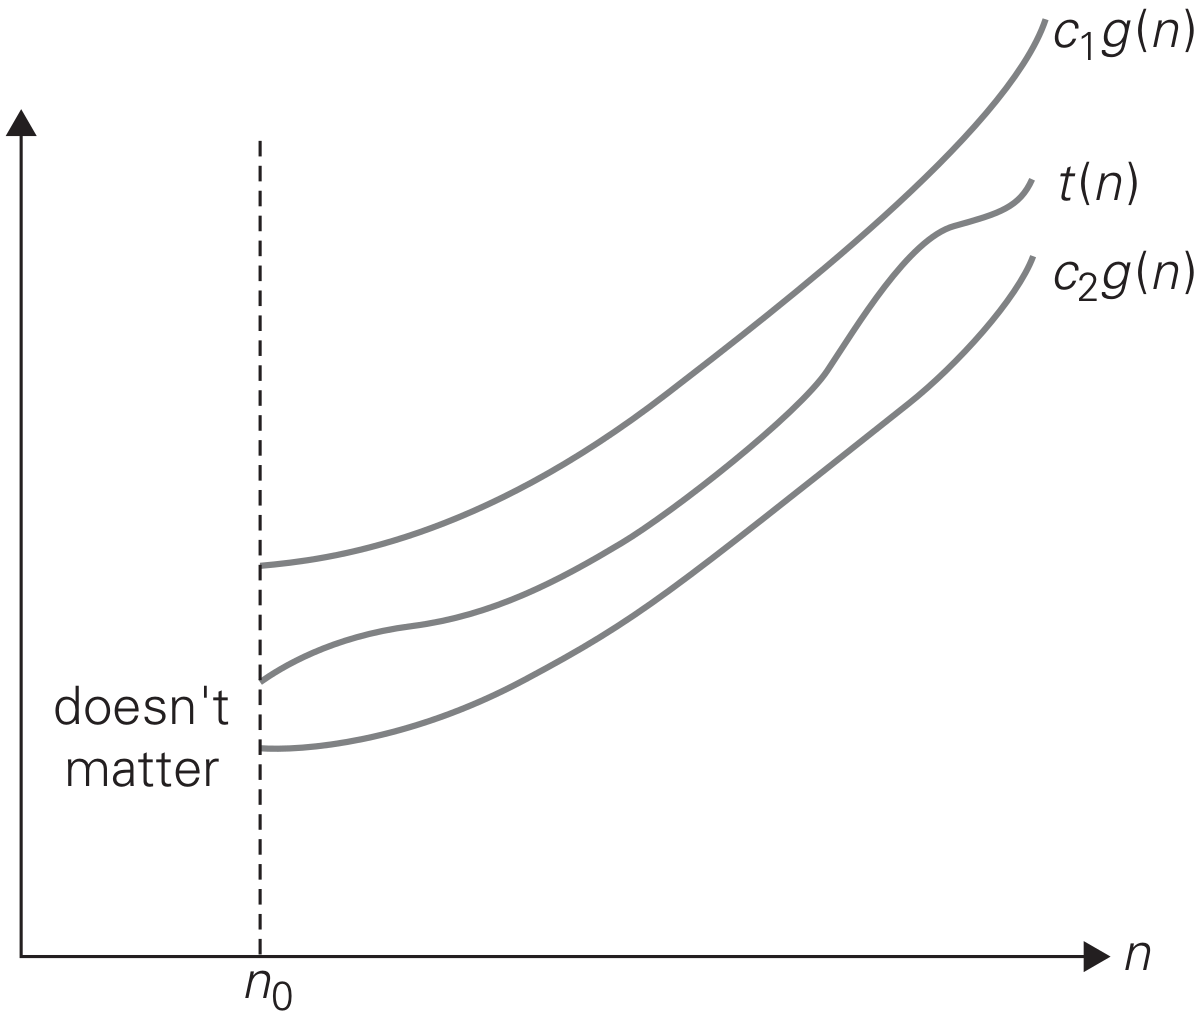
\includegraphics[width=0.5\textwidth]{big-theta_notations}
\caption{Repetition of $\Theta$-notation}
\label{fig:thetanotation}
\end{figure}

\begin{equation}
\label{eq:complexity}
C(n) = \sum_{i=0}^{n-2} \sum_{j=i+1}^{n-1} 1 \in \Theta(n^2)
\end{equation}


\textcolor{red}{In this section you must, of course, also relate to the best case, average case, and worst case input for each algorithm.}

\textcolor{red}{Do not forget to describe the results of measuring the running time and comment on them, if you opted to do this optional task.}

\lipsum[1]

\subsection{Merge Sort}
\label{sec:mergesort}

\textcolor{red}{In a subsection you describe runs of an algorithm, with graphs describing how the number of basic operation executions (on the \textit{y}-axis) varies with input size (on the \textit{x}-axis). Think carefully about the best design of the graphs, e.g. like in Fig.~\ref{fig:thetanotation}. However, you do not need to provide any execution details as they are already presented in Sec.~\ref{sec:experimentation}.}

\textcolor{red}{For each algorithm and input, you must briefly describe and explain how your empirical results relate to the theoretical results about the complexity of the algorithm (\ref{eq:complexity}). Additionally, try to identify the multiplicative constant, to be able to see more clearly which complexity class the function described by your experimental results belongs to.}

\textcolor{red}{In this section you must, of course, also relate to the best case, average case, and worst case input for each algorithm.}

\textcolor{red}{Do not forget to describe the results of measuring the running time and comment on them, if you opted to do this optional task.}

\lipsum[1-2]

\section{Conclusions}
\label{sec:conclusions}

\textcolor{red}{In this section you may want to present a few general thoughts on how the experiments went, and what you learned about the time complexity of the selected sorting algorithms.}

\lipsum[1]

\bibliographystyle{alpha}
\bibliography{levitin}

\end{document}
